\autsubsection{Debris Removal}{Lukas Christensen}
If melting is used to penetrate the Europan ice there is an issue that needs to be dealt with:\\ Experiments with ice melting probes on Earth have shown that, while they work in principle, they tend to fail after a while as debris, such as sand and dust, pile up in front of them\cite{article:di1998a}. Even in very pure ice this still becomes a problem as the debris from the entire ice column accumulate in the bottom of the bore hole as the drilling process progresses. 

\subsubsection{Debris Types}
As the exact makeup of the Europan ice sheet is still unknown it is hard to find resources detailing the types of debris that can be expected to be found during the melting process. However, at least three sources can be easily identified:\\

\begin{itemize}
	\item Surface depositions from extra-europan sources (e.g. volcanic dust from Io).
	\item Particles that were suspended in the water when the ice was formed.
	\item Meteorites.
\end{itemize}

\noindent
As described in section \ref{sec:structural_profile}, the surface of Europa appears to be covered by various pollutants like, for example, sulfur dioxide. These are thought to mainly originate from neighboring moon Io that regularly spews out volcanic dust from its frequent eruptions. While some of the deposited material will no doubt diffuse down into the ice, the majority will stay on the surface. However, simulations indicate that convection is, or at the very least has been in the past, active within in the ice sheet\cite{article:barr2014a}. This means that surface depositions may eventually work their way downwards and be distributed throughout the ice. The average size of this type of particles is likely to be on the scale of dust grains, while bigger clumps might be deposited, the process of distributing these throughout the ice is likely to decimate them into smaller pieces. \\

\noindent
If Europa has a solid core the, hopefully, liquid oceans will no doubt have been eroding it as long as water has been flowing. This means that there is likely to be a layer of a mud-like substance at the bottom of the ocean, and some of this is likely to be suspended in the oceans in colloidal form. How much of this material that is present is, however, difficult to estimate, especially considering the fact that not much is known about the current system. If life is, indeed, present in the ocean it is likely that byproducts of metabolism and decay are also suspended in the water. Through natural convection and the melting and refreezing of the lower surface of the ice sheet, these particles should over time be distributed into the ice. \\
Much like the surface depositions, it is likely that pollutants from internal sources are on the scale of dust grains, as they need to be small enough to be suspended in the water for extended periods of time.\\

\noindent
Inspecting the surface of Europa it is clear that a number of impact craters exist (see section \ref{sec:structural_profile}). Seeing as Europa have no atmosphere to speak of, meteors will arrive more or less unscathed to the surface. Of course, the rocks will be decimated upon impact, but sizable pieces will no doubt survive. As a result, larger stones must be present in the ice.  \\

\subsubsection{Removal Options}
From this basic analysis it is apparent that debris the size of dust particles are the main concern, and some method is needed to remove them for the penetrator not to get stuck. In this section, various options for dealing with this type of debris will be described. It should be noted that most of these methods will not be able to deal with rocks suspended in the ice. For that, some kind of active obstacle avoidance system is needed as will be investigated in later sections.\\

\noindent
Looking at the problem, and keeping the design of the penetrator in mind, five different methods for debris removal can be identified.
\begin{itemize}
	\item Dissolution using chemicals.
	\item Removal by a scraping device.
	\item Displacement by water jet.
	\item An ice screw system.
	\item Removal by passive means.
\end{itemize}

\noindent
The first method is seemingly simple. It would entail ejecting chemicals, such as strong acids, into the water column to dissolve the suspended debris particles. However, this is not as easy as it appears: first of all, since the exact nature of the pollutants is not known, multiple volatile chemicals would probably be needed to ensure that all can be dissolved. Not only would this require a large portion of the mass budget to be diverted to this purpose, the penetrator would likely also have to receive special anti-corrosive coatings to ensure that is won't be damaged, and this might interfere with the melting.\\

\noindent
The second option holds more promise, but it is not without issues. The basic idea is to have a mechanical device that scrapes across the front of the penetrator to move any debris to the perimeter of the bore hole. This issue with this is that, one, it requires moving mechanical parts that have to operate at the high temperature near the heater, and two, the scraping system must not obstruct the heater. Presumably, a device could be constructed such that it only scraped the heater whenever the melting progress slowed, and while this would help with the obstruction issue the complexity still makes this not ideal.\\

\noindent
The third system would consist of one ore more nozzles placed near the tip of the penetrator. By moving high pressure water through these, the resulting jet(s) would push the debris away enabling continued penetration. The water could either be deployed continuously at a fairly low pressure, or, similar to the scraping system, at a high pressure whenever the dust buildup gets too intense. Such a system would be easier to implement that the scraping system, requiring only a pump which is needed in any case to bring water samples to the different instruments. This option has been suggested for other proposed extraterrestrial thermal ice probes such as Cryobot\cite{article:zimmerman2001a}.\\

 \begin{figure}[ht]
 	\centering
 	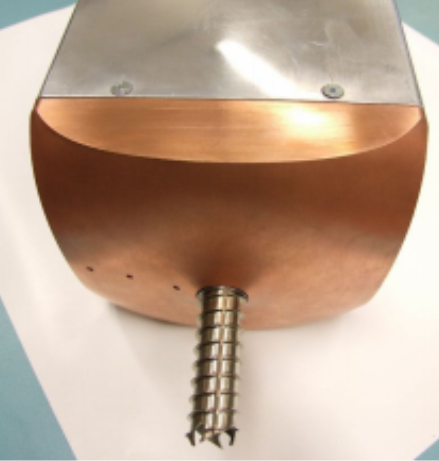
\includegraphics[width=0.45\textwidth]{figures/LAMC/iceScrew}
 	\caption{The IceMole 1 prototype using an ice screw. The copper part is the heating element and the ice screw appears in the bottom of the image. Adapted from \cite{article:dachwald2014a}}.
 	\label{fig:iceScrew}
 \end{figure}   
 
\noindent
The fourth possibility, as described by \citet{article:dachwald2014a}, works by having a screw mounted on the front of the heating element. A prototype is shown in Figure \ref{fig:iceScrew}. By rotating this screw the heater is pulled up against the ice, forcing any debris to the side. One of the big advantages of such a system is that it has a high degree of steer-ability, having even been shown to be able to move vertically upwards\cite{article:dachwald2014a}.  
Additionally, by making the screw hollow, ice cores can be made and processed inside the penetrator. Unfortunately, a number of disadvantages present themselves: The screw requires motors to rotate it, and these need to be positioned in the center of penetrator with the axle going through the heating element. This is not an issue for an electrical heater, but using RTGs in such a configuration would be very troublesome. Furthermore, in order to provide enough torque to screw into the ice, that penetrator needs to be fixed relative to the ice. \citet{article:dachwald2014a} achieve this by using a penetrator design with a square cross-section, however, this would not be ideal for Europa where the penetrator needs to be able to withstand the very high pressures experienced at the bottom of the ice sheet.\\

 \begin{figure}[ht]
 	\centering
 	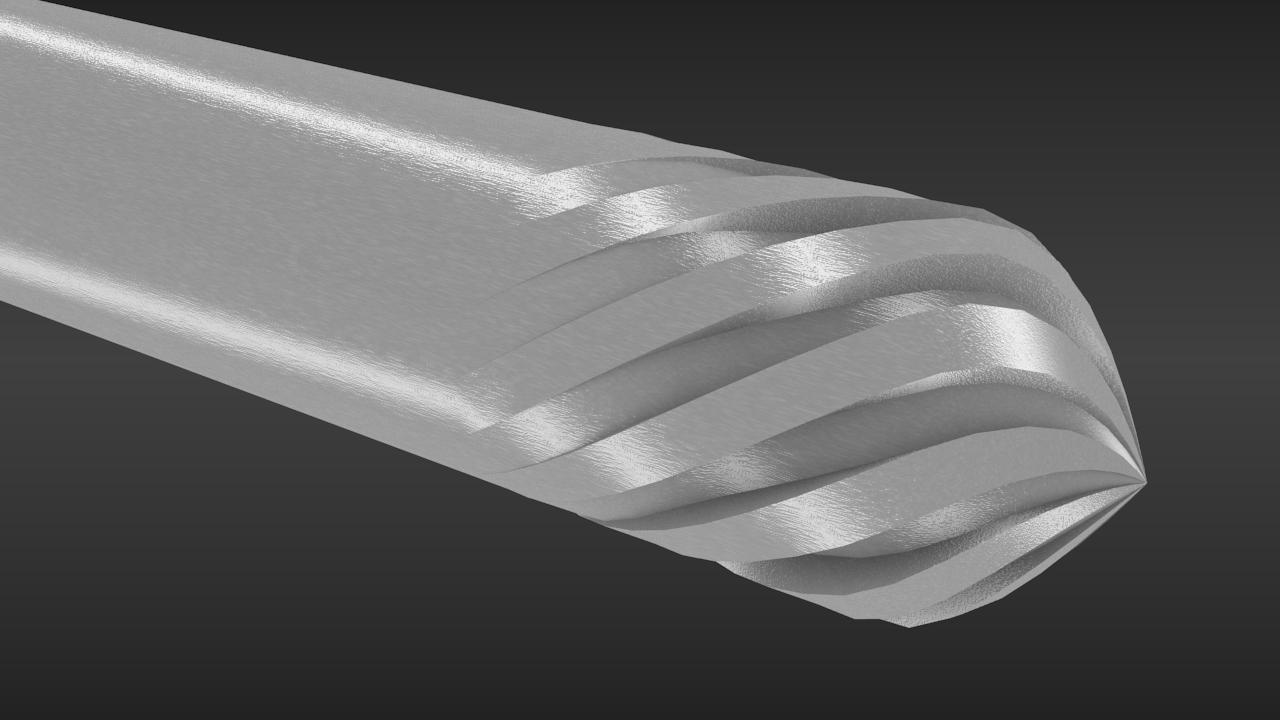
\includegraphics[width=0.5\textwidth]{figures/LAMC/flutedHead}
 	\caption{Example of how debris removal could be achieved using passive means. The flutes make the penetrator spin as it goes down, thus forcing debris to the side. This is similar to how a drill bit works.}
 	\label{fig:flutedHead}
 \end{figure}  

\noindent
The fifth method is to shape the tip of the penetrator in such a way as to remove the debris using only the motion of the penetrator itself. A way to do this is to have flutes running along the side of the device creating a shape not unlike a standard drill bit. With such a configuration, the penetrator will start to rotate as it moves downwards, and with the proper design, this will force debris to the perimeter of the bore hole following the flutes. This type of design is illustrated in Figure \ref{fig:flutedHead} and an animation ca be found at \url{https://www.youtube.com/watch?v=GRRGuUzSepY}.  \\

\noindent
Some issues that arise with this design include the fact that sharp edges do not work well with thermal melting probes, as they quickly cool down because of the large amount of heat they conduct to the surroundings. Therefore, the design in Figure \ref{fig:flutedHead} would likely have to be smoothed out somewhat, possibly reducing the debris removal efficiency. Additionally, it is hard to find examples of this design in literature, meaning that experiments are needed to determine whether it works at all. \\

\subsubsection{Discussion}
Clearly, none of these options are ideal and experiments are probably needed before a final solution can be selected. However, a combination of the third and fifth options seems like a good choice. The fluted head design causes a rotation that not only works to mitigate dust, but also works towards making the penetrator go straight down, as any unevenness that might exist in the heater will be canceled out by the rotation. This combined with the water jets is likely to be able to deal with most types of debris. \\

\noindent
If this option is chosen, it is necessary to determine the optimum number and angle of the flutes. The angle will determine the rate of rotation, and if chosen poorly it might simply stop the progress of the penetrator instead of advancing it. The number and size of the flutes will likely have an impact on how well the debris are transported away. If many small flutes are chosen it seems likely that the biggest amount of debris will be mitigated, on the other hand, the flutes cannot be so small that they cool down too quickly making the penetrator head act like a heat sink for the heating element. Of course, this is just conjecture based on educated guesses, only advanced simulations or experiments will be able to determine how it should be designed.\\

\noindent
While the flute+pump solution seems like the best choice after this initial analysis, it should not be blindly accepted. The alternatives should be exposed to a more extensive analysis to come up with values for their size, power, complexity and effectiveness before a final decision is made. A more thorough investigation into the debris types would also be beneficial. For example, if only organic compounds are found in the ice, unlikely as it may be, the chemical solution might prove to be sufficient. Similarly, if it is found that the heater can be designed to accommodate the ice screw it would provide an elegant solution. The scraping device also has its merits if an unobtrusive design can be made.\\

\noindent
Evidently, experiments and further studies are needed.   







